\documentclass[tikz,border=10pt]{standalone}
\usetikzlibrary{calc}
% Scale s = 0.022346 cm/px; origin at A, y measured upward
\begin{document}
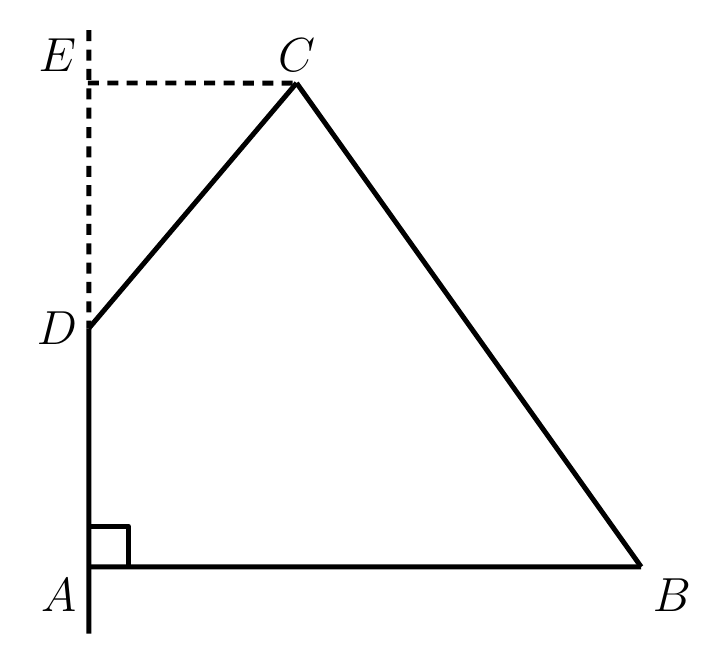
\begin{tikzpicture}[line join=round, line width=1.8pt,
  % auxiliary dashed style: dash pattern on 4pt off 3pt
  auxdash/.style={dash pattern=on 4pt off 3pt}]
  % Named coordinates (converted from pixels)
  \coordinate (A) at (0.0000019249387892550374,0.00032017997601929693);
  \coordinate (B) at (7.025996064789327,-0.00033936319416660865);
  \coordinate (C) at (2.649991653016011,6.143889939850412);
  \coordinate (D) at (0.011012352574804707,3.027990543672521);
  \coordinate (E) at (-0.0000019953189338561828,6.144138699695212);
  \coordinate (Dstub) at (0.011,-0.849);   % DA stub below A
  \coordinate (Etop) at (0.010998004681066143,6.815138699695212);     % dashed stub above E, top at y=36 px

  % Solid segments
  \draw (A) -- (B);
  \draw (B) -- (C);
  \draw (C) -- (D);
  \draw (D) -- (Dstub);

  % Dashed auxiliary segments (EC, ED and stub above E)
  \draw[auxdash] (E) -- (C);
  \draw[auxdash] (Etop) -- (D);

  % Right-angle mark at A (side about 23 px = 0.514 cm)
  \draw (0.5140019249387893,0.00032017997601929693) -- (0.5140019249387893,0.5143201799760193) -- (0.0000019249387892550374,0.5143201799760193);

  % Labels (plain math, no \boldmath)
  \node[font=\fontsize{17.5}{21}\selectfont, below left] at (A) {$A$};
  \node[font=\fontsize{17.5}{21}\selectfont, below right] at (B) {$B$};
  \node[font=\fontsize{17.5}{21}\selectfont, above] at (C) {$C$};
  \node[font=\fontsize{17.5}{21}\selectfont, left] at (D) {$D$};
  \node[font=\fontsize{17.5}{21}\selectfont, above left] at (E) {$E$};
\end{tikzpicture}
\end{document}
% GEOAGENT_REPAIR_V1 c18a466396f54661 827c2b4e0bf4eb824d13e70a53c82f84c763909d9e19f05ade516721437589d1
